\documentclass{article}

\def\npart{III}
\def\nyear{2018}
\def\nterm{Michaelmas}
\def\nlecturer{Dr. S. Barbina}
\def\ncourse{Model Theory}
\def\draft{Ongoing course, rough}
\usepackage{mathrsfs}
\usepackage{imakeidx}
\ifx \nauthor\undefined
  \def\nauthor{Bhavik Mehta}
\else
\fi

\author{Based on lectures by \nlecturer \\\small Notes taken by \nauthor}
\date{\nterm\ \nyear}
\title{Part \npart\ -- \ncourse}

\usepackage[utf8]{inputenc}
\usepackage{amsmath}
\usepackage{amsthm}
\usepackage{amssymb}
\usepackage{enumerate}
\usepackage{mathtools}
\usepackage{graphicx}
\usepackage[dvipsnames]{xcolor}
\usepackage{tikz}
\usepackage{wrapfig}
\usepackage{centernot}
\usepackage{float}
\usepackage{braket}
\usepackage[hypcap=true]{caption}
\usepackage{enumitem}
\usepackage[colorlinks=true, linkcolor=mblue]{hyperref}
\usepackage[nameinlink,noabbrev]{cleveref}
\usepackage{nameref}
\usepackage[margin=1.5in]{geometry}

% Theorems
\theoremstyle{definition}
\newtheorem*{aim}{Aim}
\newtheorem*{axiom}{Axiom}
\newtheorem*{claim}{Claim}
\newtheorem*{cor}{Corollary}
\newtheorem*{conjecture}{Conjecture}
\newtheorem*{defi}{Definition}
\newtheorem*{eg}{Example}
\newtheorem*{ex}{Exercise}
\newtheorem*{fact}{Fact}
\newtheorem*{law}{Law}
\newtheorem*{lemma}{Lemma}
\newtheorem*{notation}{Notation}
\newtheorem*{prop}{Proposition}
\newtheorem*{question}{Question}
\newtheorem*{rrule}{Rule}
\newtheorem*{thm}{Theorem}
\newtheorem*{assumption}{Assumption}

\newtheorem*{remark}{Remark}
\newtheorem*{warning}{Warning}
\newtheorem*{exercise}{Exercise}

% \newcommand{\nthmautorefname}{Theorem}

\newtheorem{nthm}{Theorem}[section]
\newtheorem{nlemma}[nthm]{Lemma}
\newtheorem{nprop}[nthm]{Proposition}
\newtheorem{ncor}[nthm]{Corollary}
\newtheorem{ndef}[nthm]{Definition}

% Special sets
\newcommand{\C}{\mathbb{C}}
\newcommand{\N}{\mathbb{N}}
\newcommand{\Q}{\mathbb{Q}}
\newcommand{\R}{\mathbb{R}}
\newcommand{\Z}{\mathbb{Z}}

\newcommand{\abs}[1]{\left\lvert #1\right\rvert}
\newcommand{\norm}[1]{\left\lVert #1\right\rVert}
\renewcommand{\vec}[1]{\boldsymbol{\mathbf{#1}}}

\let\Im\relax
\let\Re\relax

\DeclareMathOperator{\Im}{Im}
\DeclareMathOperator{\Re}{Re}
\DeclareMathOperator{\id}{id}

\definecolor{mblue}{rgb}{0., 0.05, 0.6}

\makeindex[intoc]

% preamble

\setcounter{section}{-1}

\DeclarePairedDelimiter\ceil{\lceil}{\rceil}
\DeclarePairedDelimiter\floor{\lfloor}{\rfloor}

\newtheorem{nremark}[nthm]{Remark}
\newtheorem{nexample}[nthm]{Example}
\newtheorem{nexercise}[nthm]{Exercise}

%\newtheorem{manualtheoreminner}{Theorem}
%\newenvironment{manualtheorem}[1]{%
%    \renewcommand\themanualtheoreminner{#1}%
%    \manualtheoreminner
%}{\endmanualtheoreminner}

%\newcommand{\red}[1]{\textcolor{bred}{#1}}
%\newcommand{\green}[1]{\textcolor{bgreen}{#1}}
%\newcommand{\blue}[1]{\textcolor{bblue}{#1}}
%\newcommand{\yellow}[1]{\textcolor{byellow}{#1}}
%\newcommand{\orange}[1]{\textcolor{borange}{#1}}
%\newcommand{\purple}[1]{\textcolor{bpurple}{#1}}

% and here we go!

\begin{document}
\maketitle

\tableofcontents

\clearpage
\section{Introduction}
Model theory is a part of logic that began by looking at algebraic objects such as groups and combinatorial objects such like graphs, described in formal language.
The basic question in model theory is: `how powerful is our description of these objects to pin them down'?
In Logic and Set Theory, the focus was on what was provable from a theory and language, but here we focus on whether or not a model exists.

\section{Languages and structures}
\begin{ndef}[Language]\index{language}\hypertarget{def:lang}
  A \textbf{language} $L$ consists of
  \begin{enumerate}[label=(\roman*)]
    \item a set $\mathscr{F}$ of function symbols, and for each $f \in \mathscr{F}$ a positive integer $m_f$ the \textbf{arity} of $f$.
    \item a set $\mathscr{R}$ of relation symbols, and for each $R \in \mathscr{R}$, a positive integer $m_R$.
    \item a set $\mathscr{C}$ of constant symbols.
  \end{enumerate}
  Note: each of $\mathscr{F}, \mathscr{R}$ and $\mathscr{C}$ can be empty.
\end{ndef}
\begin{eg}
  \hypertarget{def:lgp}Take $L = \{\{\cdot , ^{-1}\}, \{1\}\}$, for $\cdot$ a binary function and $^{-1}$ an unary function, $1$ a constant. This is the \hyperlink{def:lang}{language} of groups, call it $L_{gp}$.
  Also, $L_{lo} = \{<\}$ a single binary relation, for linear orders.
\end{eg}

\begin{ndef}[$L$-structure]\index{$L$-structure}\hypertarget{def:lstr}
  Given a \hyperlink{def:lang}{language} $L$, say, an \textbf{$L$-structure} consists of
  \begin{enumerate}[label=(\roman*)]
    \item a set $M$, the \textbf{domain}
    \item for each $f \in \mathscr{F}$, a function $f^\mathcal{M} : M^{m_f} \to M$.
    \item for each $R \in \mathscr{R}$, a relation $R^\mathcal{M} \subseteq M^{m_R}$.
    \item for each $c \in \mathscr{C}$, an element $c^\mathcal{M} \in M$.
  \end{enumerate}
  $f^M, R^M, c^M$ are the \textbf{interpretations} of $f,R,c$ respectively.
\end{ndef}
\begin{nremark}
  We often fail to distinguish between the \hyperlink{def:lang}{symbols} in $L$ and their \hyperlink{def:lstr}{interpretations} in a \hyperlink{def:lstr}{structure}, if the interpretations are clear from the context.
\end{nremark}

We may write $\mathcal{M} = \langle M, \mathscr{F}, \mathscr{R}, \mathscr{C} \rangle$.

\begin{nexample}\leavevmode
  \begin{enumerate}[label=(\alph*)]
    \item $\mathcal{R} = \langle \mathbb{R}^+, \{\cdot, ^{-1}\}, 1 \rangle$ is an \hyperlink{def:lgp}{$L_{gp}$}-\hyperlink{def:lstr}{structure}.
    \item $\mathcal{Z} = \langle \mathbb{Z}, \{+, -\}, 0 \rangle$ is an $L_{gp}$-structure.
    \item $\mathcal{Q} = \langle \mathbb{Q}, < \rangle$ is an \hyperlink{def:lgp}{$L_{lo}$}-structure.
  \end{enumerate}
\end{nexample}
\begin{ndef}[Embedding]\label{def:1.5}\index{embedding}\hypertarget{def:embedding}
  Let $L$ be a \hyperlink{def:language}{language}, let $\mathcal{M}, \mathcal{N}$ be \hyperlink{def:lstr}{$L$-structures}.
  An \textbf{embedding} of $\mathcal{M}$ into $\mathcal{N}$ is a one-to-one mapping $\alpha: M \to N$ such that
  \begin{enumerate}[label=(\roman*)]
    \item for all $f \in \mathscr{F}$, and $a_1, \dotsc, a_{m_f} \in M$,
      \begin{equation*}
        \alpha(f^\mathcal{M}(a_1, \dotsc, a_{n_f})) = f^\mathcal{N}(\alpha(a_1), \dotsc, \alpha(a_{n_f}))
      \end{equation*}
      \begin{center}
        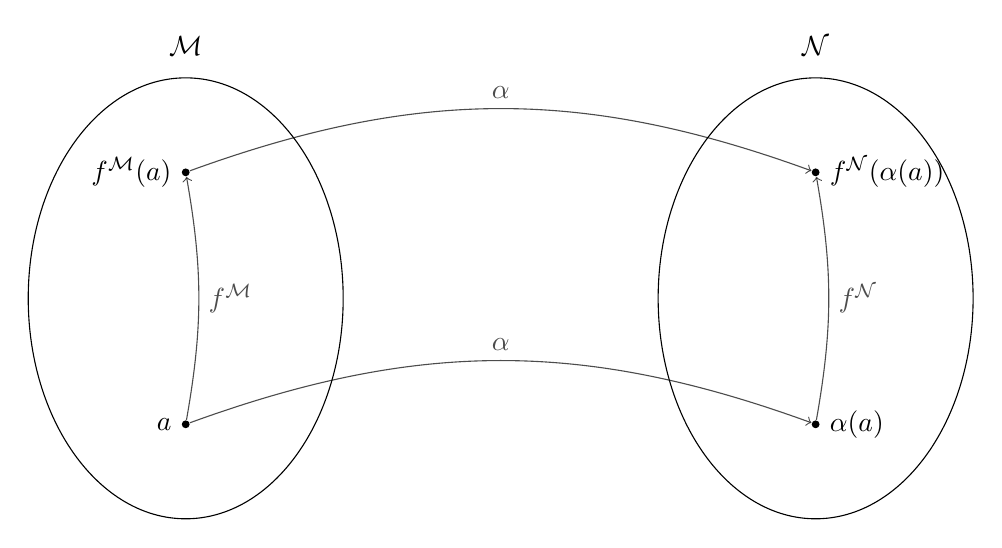
\begin{tikzpicture}[scale=2]
          \node at (-2, 1.6) {$\mathcal{M}$};
          \node at (2, 1.6) {$\mathcal{N}$};
          \draw (-2, 0) circle [x radius=10mm, y radius=14mm];
          \node [circle, inner sep=1pt, fill=black, label=left:$a$] (a) at (-2, -0.8) {};
          \node [circle, inner sep=1pt, fill=black, label=left:$f^\mathcal{M}(a)$] (fa) at (-2, 0.8) {};
          \draw (2, 0) circle [x radius=10mm, y radius=14mm];
          \node [circle, inner sep=1pt, fill=black, label=right:$\alpha(a)$] (aa) at (2, -0.8) {};
          \node [circle, inner sep=1pt, fill=black, label=right:$f^\mathcal{N}(\alpha(a))$] (faa) at (2, 0.8) {};
          \draw [->, opacity=0.7] (a) to [bend left=20] node[above]{$\alpha$} (aa);
          \draw [->, opacity=0.7] (fa) to [bend left=20] node[above]{$\alpha$} (faa);
          \draw [->, opacity=0.7] (a) to [bend right=10] node[right]{$f^\mathcal{M}$} (fa);
          \draw [->, opacity=0.7] (aa) to [bend right=10] node[right]{$f^\mathcal{N}$} (faa);
        \end{tikzpicture}
      \end{center}
    \item for all $R \in \mathscr{R}$, and $a_1, \dotsc, a_{n_R} \in M$
      \begin{equation*}
        (a_1, \dotsc, a_{n_R}) \in R^\mathcal{M} \iff (\alpha(a_1), \dotsc, \alpha(a_{n_R})) \in R^\mathcal{N}
      \end{equation*}
    \item for all $c \in \mathscr{C}$, $\alpha(c^\mathcal{M}) = c^\mathcal{N}$.
  \end{enumerate}
  An \textbf{isomorphism} of $\mathcal{M}$ into $\mathcal{N}$ is a surjective embedding (onto).
\end{ndef}

\begin{nexercise}
  Let $G_1, G_2$ be groups, regarded as $L_{gp}$-structures. Check that $G_1 \simeq G_2$ in the usual algebra sense if and only if there is an isomorphism $\alpha: G_1 \to G_2$ in the sense of \cref{def:1.5}
\end{nexercise}

\section{Review: Terms, formulae and their interpretations}
In addition to the symbols of $L$, we also have
\begin{enumerate}[label=(\roman*)]
  \item infinitely many variables $\{x_i\}_{i \in I}$
  \item logical connectives $\wedge, \neg$ (also expresses $\vee, \Rightarrow, \iff$)
    \item quantifier $\exists$ (also expresses $\forall$)
    \item $(\phantom{\cdot},\phantom{\cdot})$
\end{enumerate}

\begin{ndef}[\hypertarget{def:lterm}{$L$-terms}]
  \index{$L$-term}\textbf{$L$-terms} are defined recursively as follows:
  \begin{itemize}[label=--]
    \item any variable $x_i$ is a term
    \item any constant symbol is a term
    \item for any $f \in \mathscr{F}$, $f(t_1, \dotsc, t_{m_f})$ for any terms $t_1, \dotsc, t_{m_f}$ is a term
    \item nothing else is a term
  \end{itemize}
\end{ndef}

Notation: we write $t(x_1, \dotsc, x_m)$ to mean that the variables appearing in $t$ are among $x_1, \dotsc, x_m$.
\begin{eg}
  Take $\mathcal{R} = \langle \mathbb{R}^*, \{\cdot, ^{-1}\}, 1 \rangle$. Then $\cdot ( \cdot(x_1, x_2), x_3)$ is a term, usually written $(x_1 \cdot x_2) \cdot x_3$. Also, $(\cdot (1, x_1))^{-1}$ is a term, written $(1\cdot x)^{-1}$
\end{eg}
\begin{ndef}
  If $\mathcal{M}$ is an $L$-structure, to each $L$-term $t(x_1, \dotsc, x_k)$ we assign a function
  a function $t^\mathcal{M}: M^k \to M$ defined as follows:
  \begin{enumerate}[label=(\roman*)]
    \item If $t = x_i$, $t^\mathcal{M}[a_1, \dotsc, a_k] = a_i$
    \item If $t = c$, $t^\mathcal{M}[a_1, \dotsc, a_k] = c^\mathcal{M}$.
    \item If $t = f(t(x_1, \dotsc, x_k), \dotsc, t_{m_f}(x_1, \dotsc, x_k))$,
      \begin{equation*}
        t^\mathcal{M}(a_1, \dotsc, a_k) = f^\mathcal{M}(t_1^\mathcal{M}(a_1, \dotsc, a_k), \dotsc, t^\mathcal{M}_{m_f}(a_1, \dotsc, a_k))
      \end{equation*}
  \end{enumerate}
\end{ndef}
\end{document}
